\chapter{Liste der implementierten Klassen und Methoden}
\label{appendix:classes}
\section{dll.py}

\begin{itemize}

    \item \texttt{Leaf}: Ein Element einer doppelt verketteten List mit den Attributen \texttt{key}, \texttt{value}, \texttt{prev} und \texttt{succ}

    \begin{itemize}
        \item \texttt{insertAfter}: Fügt ein Objekt nach dem Objekt ein
        \item \texttt{insertBefore}: Fügt ein Objekt vor dem Objekt ein
        \item \texttt{remove}: Entfernt das Objekt
    \end{itemize}

    \item \texttt{DoublyLinkedList}: Eine doppelt verkettete Liste, enthält die Referenz zum Dummy Element mit dem Schlüssel $\infty$

    \begin{itemize}
        \item \texttt{locate}: Findet das Element mit dem gesuchten Schlüssel
        \item \texttt{insert}: Fügt ein Element mit dem gegebenen Schlüssel ein
        \item \texttt{remove}: Entfernt das Element mit dem gegebenen Schlüssel
        \item \texttt{isEmpty}: Prüft Liste auf Leere
        \item \texttt{first}: Gibt erstes Element zurück
        \item \texttt{last}: Gibt letztes Element zurück
        \item \texttt{count}: Gibt Anzahl der Elemente in der Liste zurück
    \end{itemize}

\end{itemize}

\section{abTree.py}

\begin{itemize}

    \item \texttt{Node}
    \item \texttt{ABTree}

\end{itemize}

\chapter{weitere Testergebnisse}
\label{appendix:benchmarks}

\begin{figure}
    \centering{
        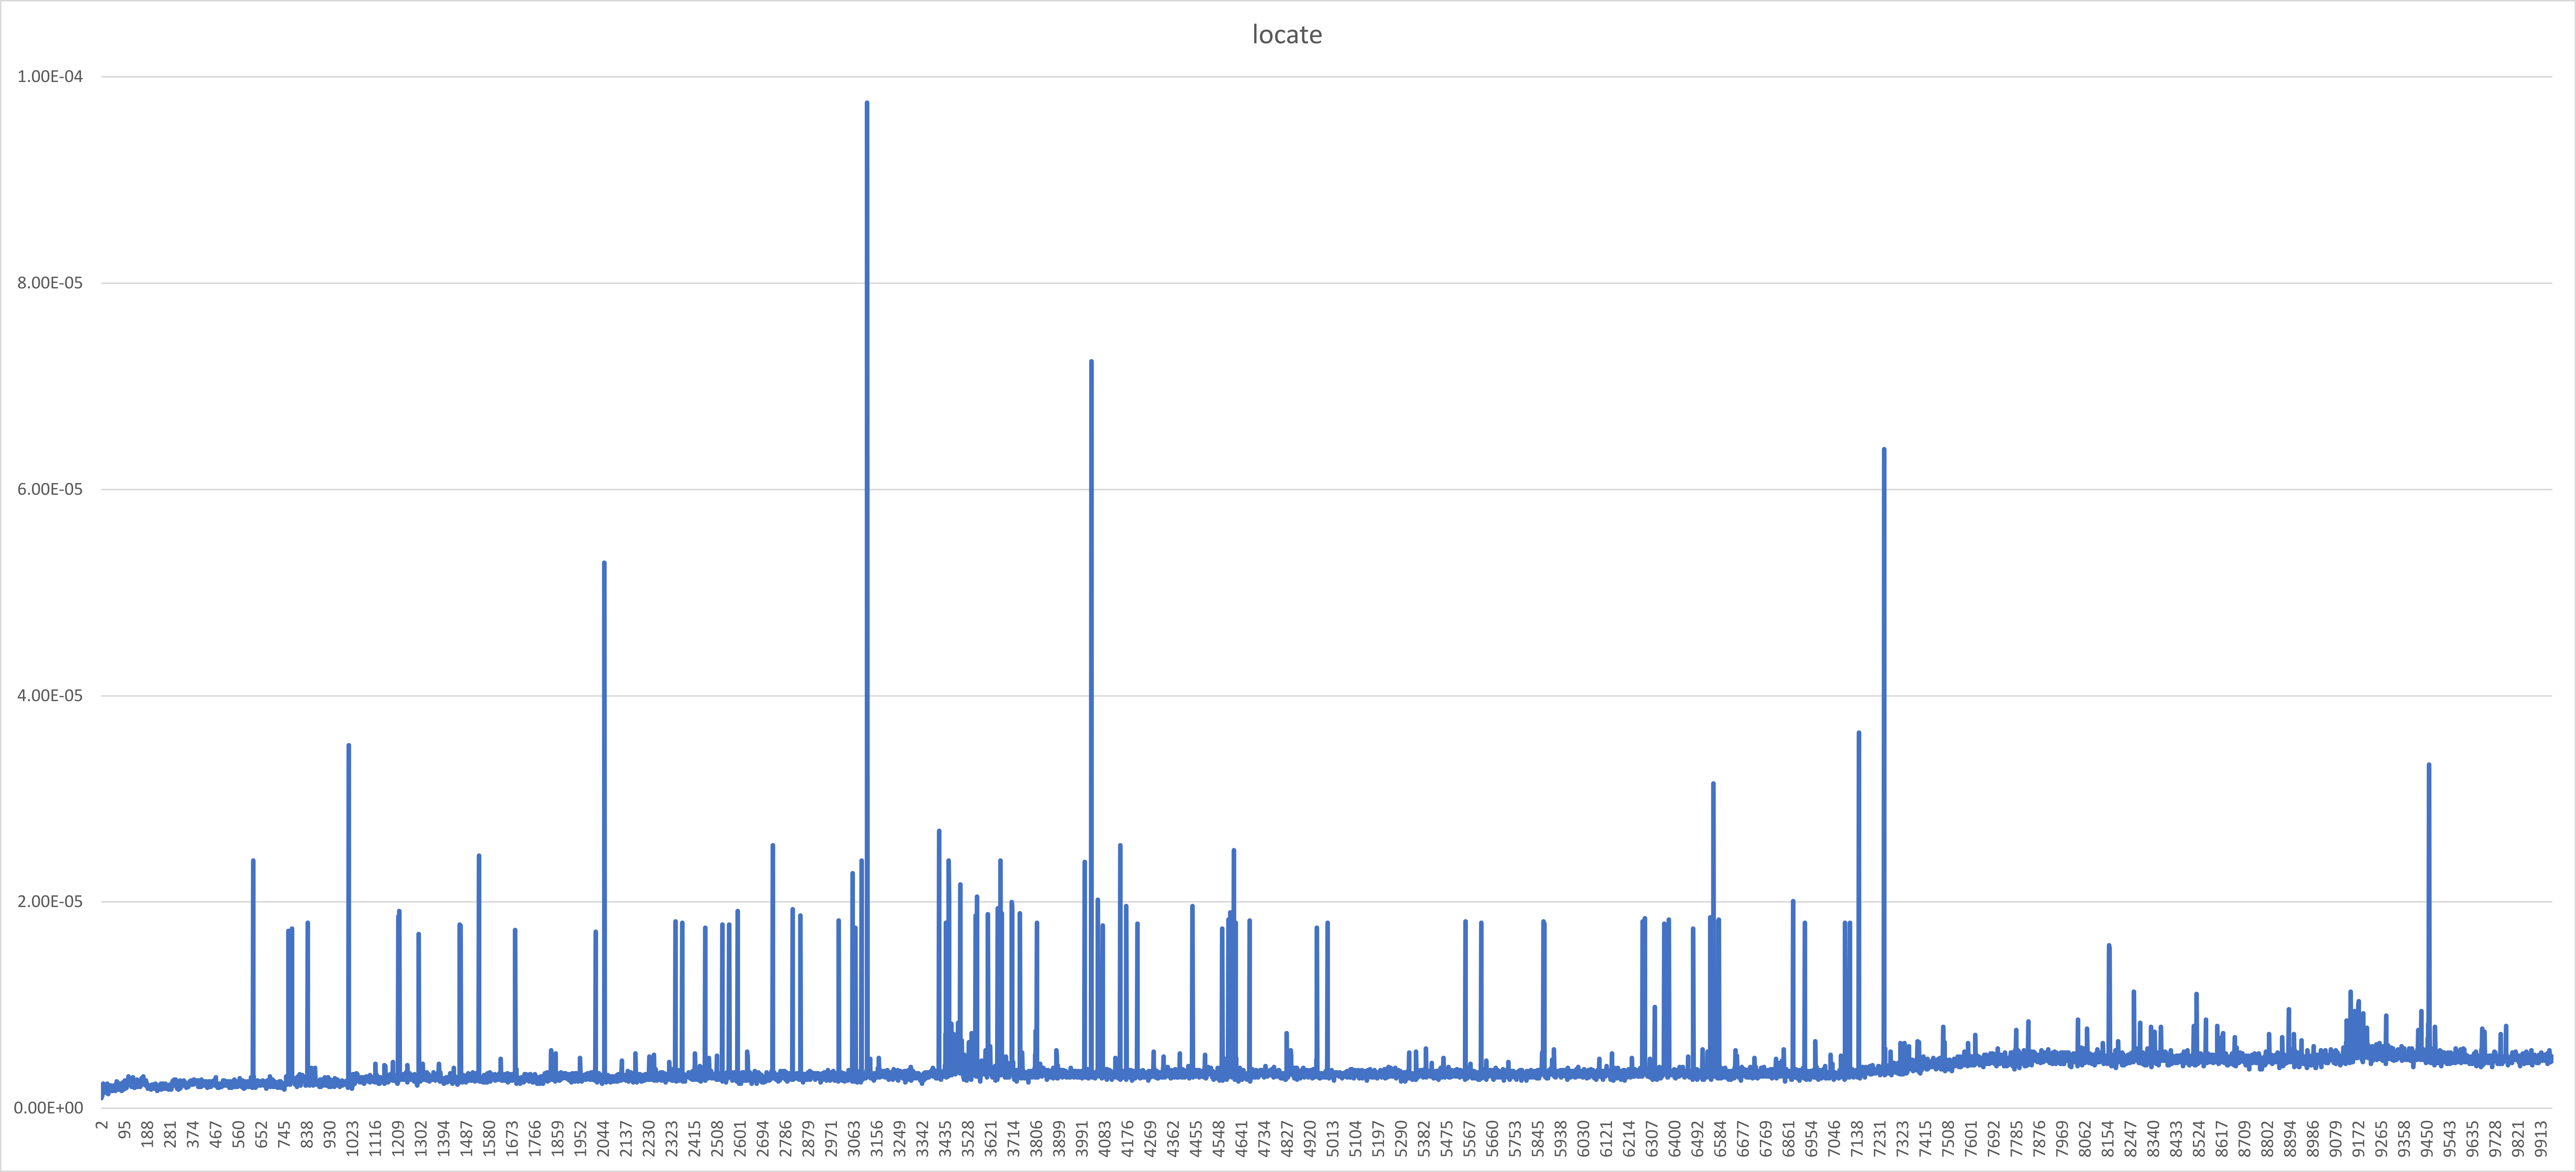
\includegraphics[width=\linewidth]{assets/benchmark10raw.png}
        \caption{Die unbearbeiteten Ergebnisse des Tests an einer sortierten Sequenz mit maximal 10.000 Elementen. Dargestellt ist die Dauer der Funktion \texttt{locate}. Durch die großen Messspitzen sind die Ergebnisse nicht gut ablesbar.}
        \label{fig:benchmark10raw}
    }
\end{figure}

\begin{figure}
    \centering{
        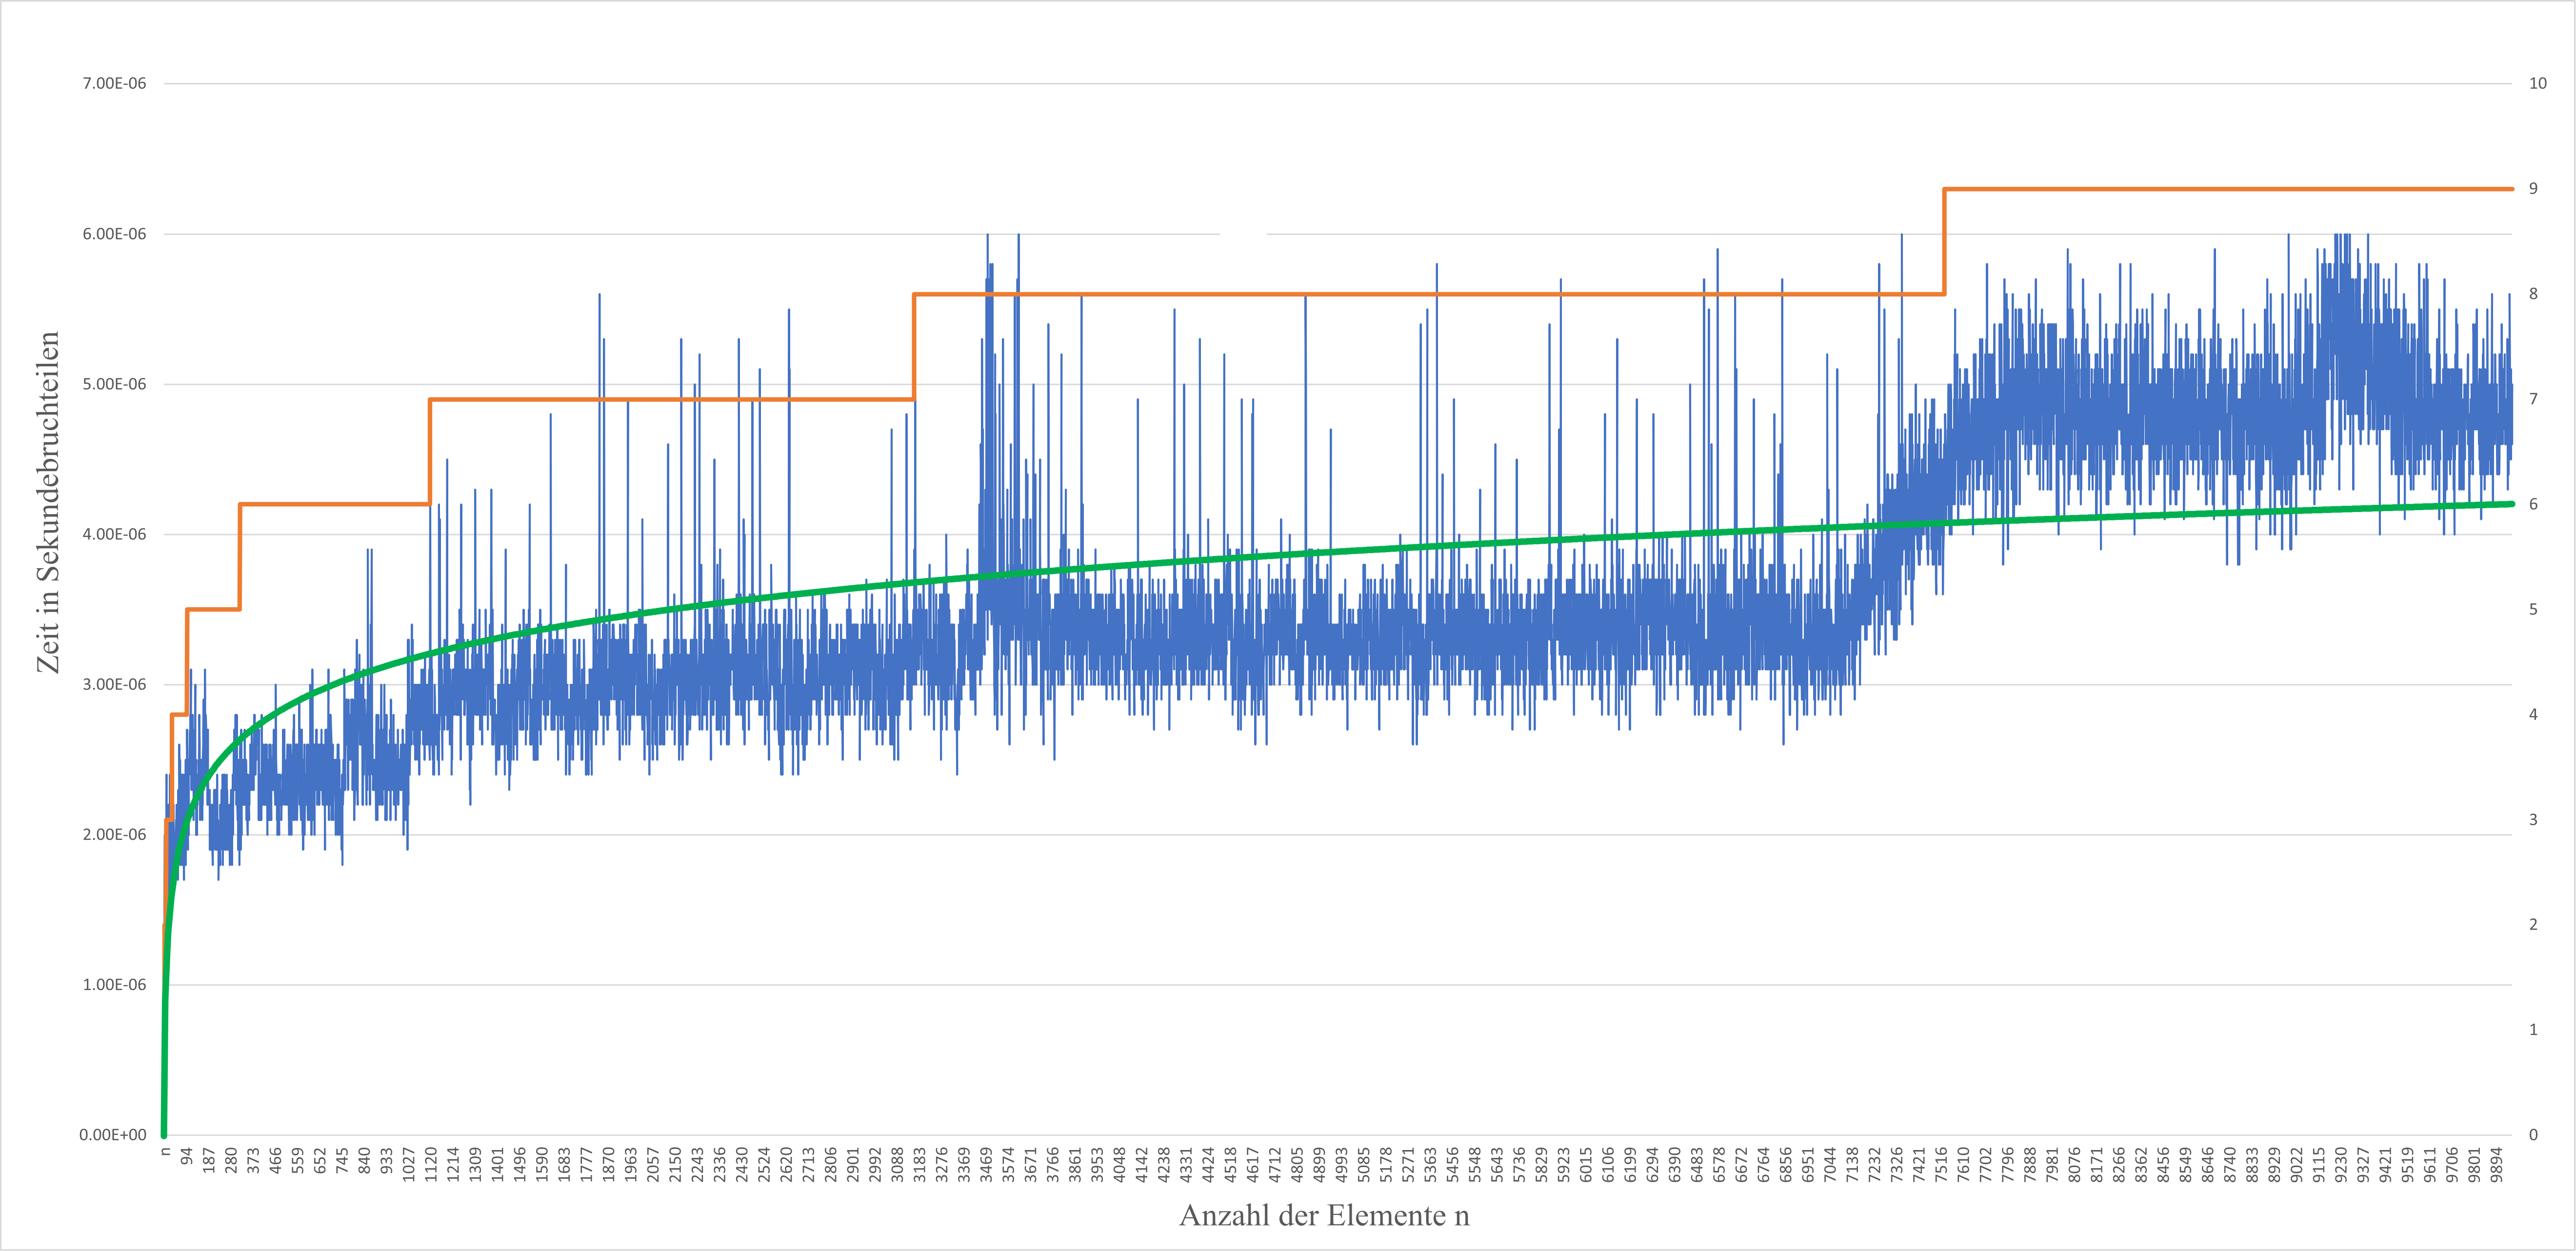
\includegraphics[width=\linewidth]{assets/benchmark10.png}
        \caption{Die bearbeiteten Ergebnisse des Testes mit 10.000 Elementen zeigen die logarithmische Laufzeit von \texttt{locate}, sowie die Abhängigkeit von der Höhe des Baumes (orange dargestellt)}
        \label{fig:benchmark10}
    }
\end{figure}

\begin{figure}
    \centering{
        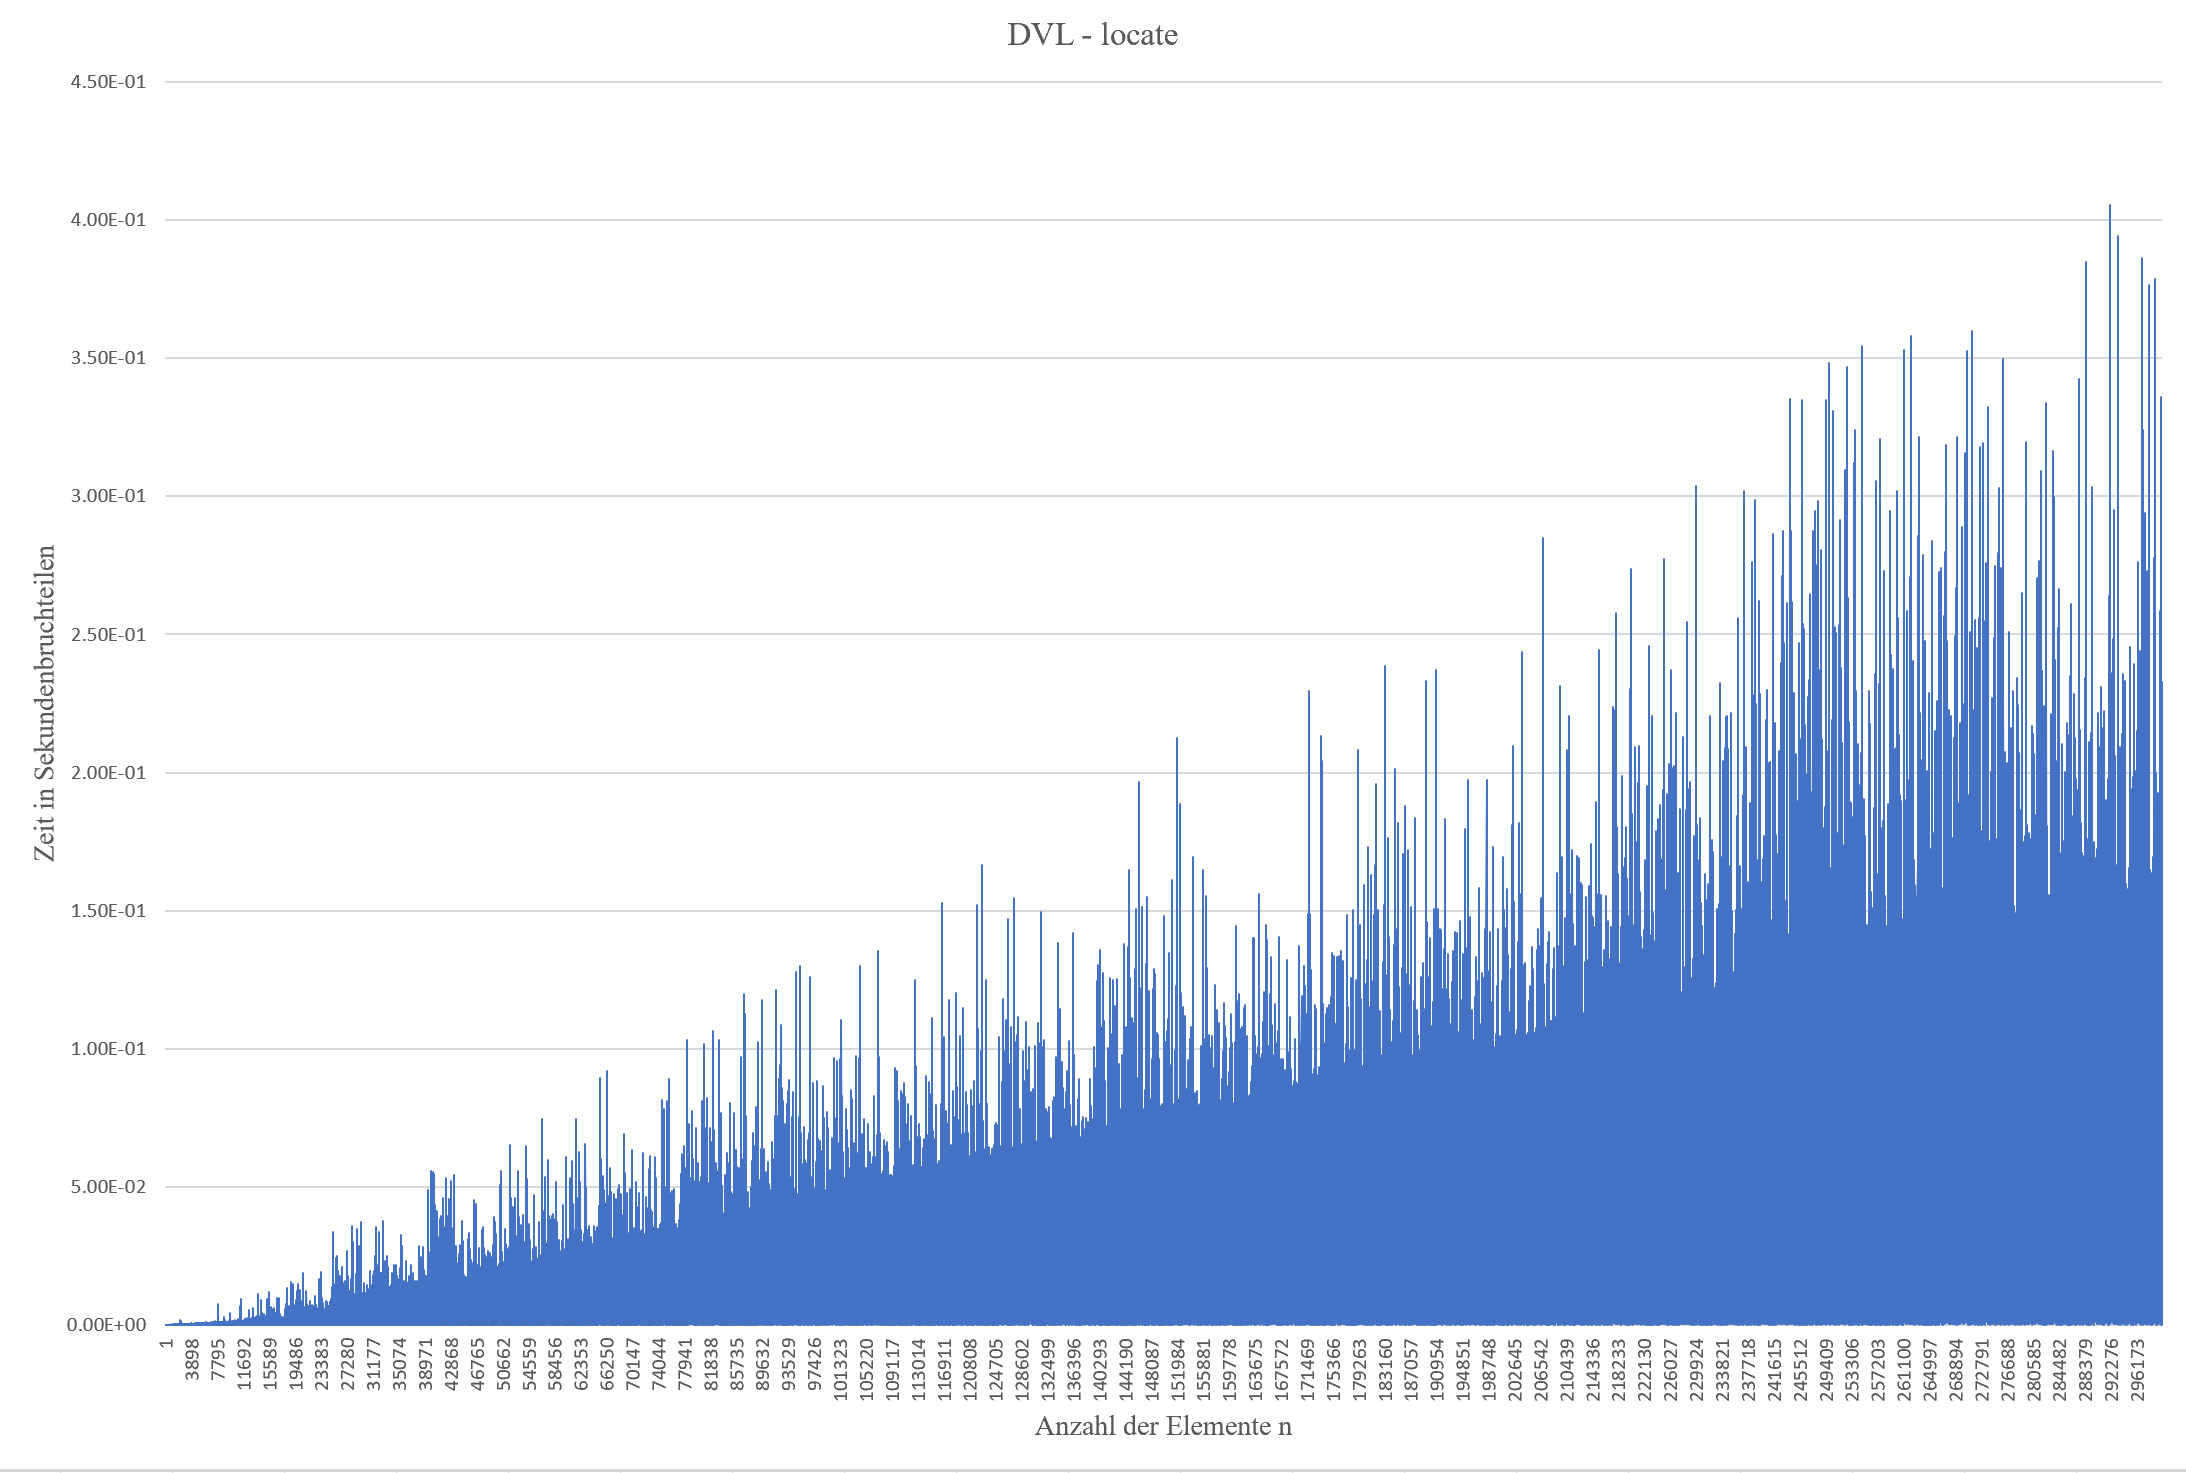
\includegraphics[width=\linewidth]{assets/benchlist.png}
        \caption{Die unbearbeiteten Ergebnisse des Tests an einer Doppelt Verketteten List (DVL) mit maximal 300.000 Elementen. Dargestellt ist die Dauer der Funktion \texttt{locate}. Die Messspitzen lenken hier weniger vom Ergebnis ab als bei (a,b)-Bäumen. Die lineare Laufzeit ist deutlich erkennbar.}
        \label{fig:benchmark10raw}
    }
\end{figure}
